\documentclass[1p]{elsarticle_modified}
%\bibliographystyle{elsarticle-num}

%\usepackage[colorlinks]{hyperref}
%\usepackage{abbrmath_seonhwa} %\Abb, \Ascr, \Acal ,\Abf, \Afrak
\usepackage{amsfonts}
\usepackage{amssymb}
\usepackage{amsmath}
\usepackage{amsthm}
\usepackage{scalefnt}
\usepackage{amsbsy}
\usepackage{kotex}
\usepackage{caption}
\usepackage{subfig}
\usepackage{color}
\usepackage{graphicx}
\usepackage{xcolor} %% white, black, red, green, blue, cyan, magenta, yellow
\usepackage{float}
\usepackage{setspace}
\usepackage{hyperref}

\usepackage{tikz}
\usetikzlibrary{arrows}

\usepackage{multirow}
\usepackage{array} % fixed length table
\usepackage{hhline}

%%%%%%%%%%%%%%%%%%%%%
\makeatletter
\renewcommand*\env@matrix[1][\arraystretch]{%
	\edef\arraystretch{#1}%
	\hskip -\arraycolsep
	\let\@ifnextchar\new@ifnextchar
	\array{*\c@MaxMatrixCols c}}
\makeatother %https://tex.stackexchange.com/questions/14071/how-can-i-increase-the-line-spacing-in-a-matrix
%%%%%%%%%%%%%%%

\usepackage[normalem]{ulem}

\newcommand{\msout}[1]{\ifmmode\text{\sout{\ensuremath{#1}}}\else\sout{#1}\fi}
%SOURCE: \msout is \stkout macro in https://tex.stackexchange.com/questions/20609/strikeout-in-math-mode

\newcommand{\cancel}[1]{
	\ifmmode
	{\color{red}\msout{#1}}
	\else
	{\color{red}\sout{#1}}
	\fi
}

\newcommand{\add}[1]{
	{\color{blue}\uwave{#1}}
}

\newcommand{\replace}[2]{
	\ifmmode
	{\color{red}\msout{#1}}{\color{blue}\uwave{#2}}
	\else
	{\color{red}\sout{#1}}{\color{blue}\uwave{#2}}
	\fi
}

\newcommand{\Sol}{\mathcal{S}} %segment
\newcommand{\D}{D} %diagram
\newcommand{\A}{\mathcal{A}} %arc


%%%%%%%%%%%%%%%%%%%%%%%%%%%%%5 test

\def\sl{\operatorname{\textup{SL}}(2,\Cbb)}
\def\psl{\operatorname{\textup{PSL}}(2,\Cbb)}
\def\quan{\mkern 1mu \triangleright \mkern 1mu}

\theoremstyle{definition}
\newtheorem{thm}{Theorem}[section]
\newtheorem{prop}[thm]{Proposition}
\newtheorem{lem}[thm]{Lemma}
\newtheorem{ques}[thm]{Question}
\newtheorem{cor}[thm]{Corollary}
\newtheorem{defn}[thm]{Definition}
\newtheorem{exam}[thm]{Example}
\newtheorem{rmk}[thm]{Remark}
\newtheorem{alg}[thm]{Algorithm}

\newcommand{\I}{\sqrt{-1}}
\begin{document}

%\begin{frontmatter}
%
%\title{Boundary parabolic representations of knots up to 8 crossings}
%
%%% Group authors per affiliation:
%\author{Yunhi Cho} 
%\address{Department of Mathematics, University of Seoul, Seoul, Korea}
%\ead{yhcho@uos.ac.kr}
%
%
%\author{Seonhwa Kim} %\fnref{s_kim}}
%\address{Center for Geometry and Physics, Institute for Basic Science, Pohang, 37673, Korea}
%\ead{ryeona17@ibs.re.kr}
%
%\author{Hyuk Kim}
%\address{Department of Mathematical Sciences, Seoul National University, Seoul 08826, Korea}
%\ead{hyukkim@snu.ac.kr}
%
%\author{Seokbeom Yoon}
%\address{Department of Mathematical Sciences, Seoul National University, Seoul, 08826,  Korea}
%\ead{sbyoon15@snu.ac.kr}
%
%\begin{abstract}
%We find all boundary parabolic representation of knots up to 8 crossings.
%
%\end{abstract}
%\begin{keyword}
%    \MSC[2010] 57M25 
%\end{keyword}
%
%\end{frontmatter}

%\linenumbers
%\tableofcontents
%
\newcommand\colored[1]{\textcolor{white}{\rule[-0.35ex]{0.8em}{1.4ex}}\kern-0.8em\color{red} #1}%
%\newcommand\colored[1]{\textcolor{white}{ #1}\kern-2.17ex	\textcolor{white}{ #1}\kern-1.81ex	\textcolor{white}{ #1}\kern-2.15ex\color{red}#1	}

{\Large $\underline{12a_{0061}~(K12a_{0061})}$}

\setlength{\tabcolsep}{10pt}
\renewcommand{\arraystretch}{1.6}
\vspace{1cm}\begin{tabular}{m{100pt}>{\centering\arraybackslash}m{274pt}}
\multirow{5}{120pt}{
	\centering
	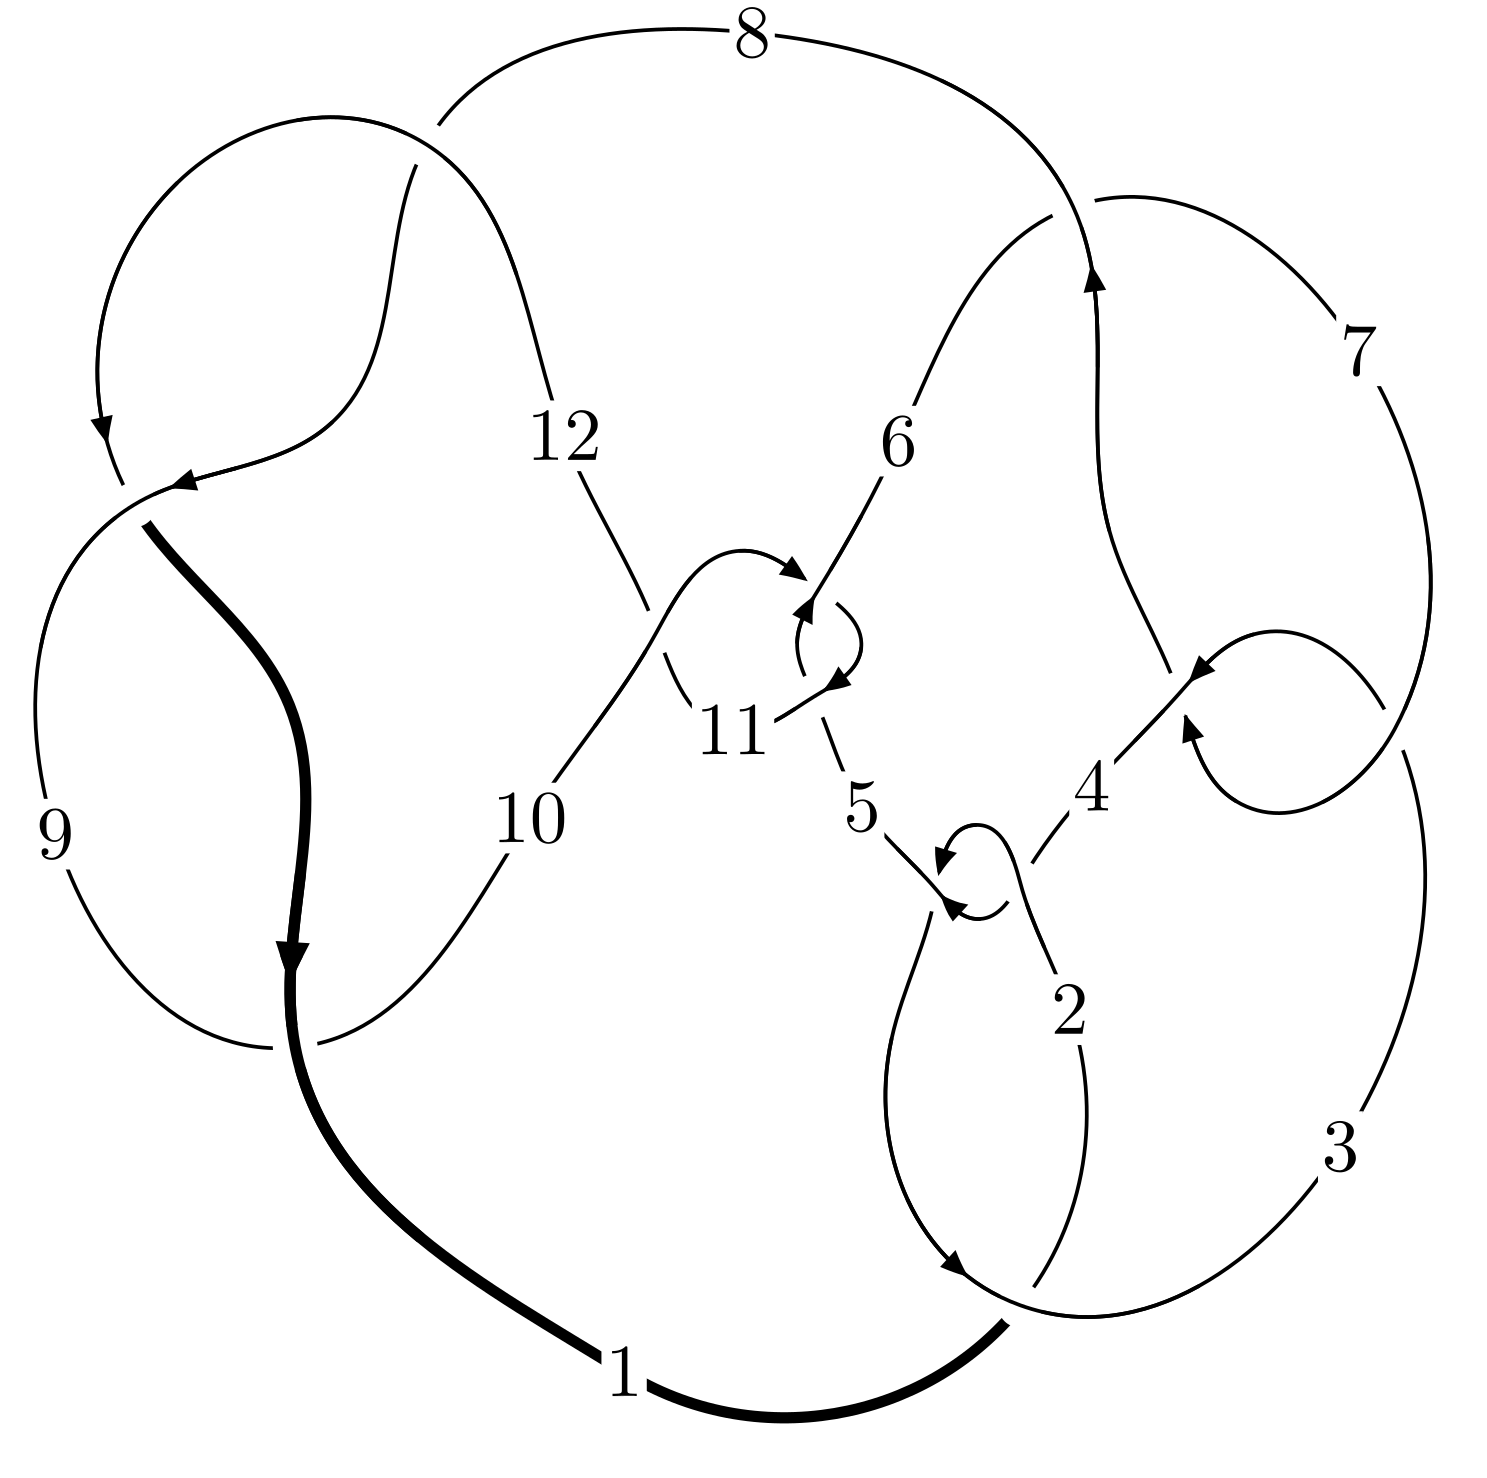
\includegraphics[width=112pt]{../../../GIT/diagram.site/Diagrams/png/862_12a_0061.png}\\
\ \ \ A knot diagram\footnotemark}&
\allowdisplaybreaks
\textbf{Linearized knot diagam} \\
\cline{2-2}
 &
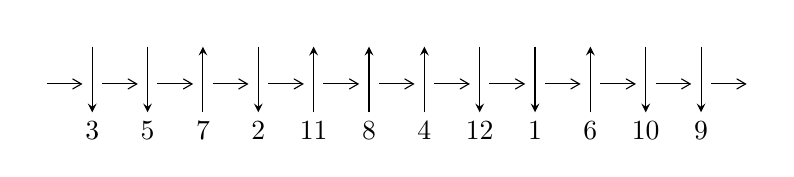
\begin{tikzpicture}[x=20pt, y=17pt]
	% nodes
	\node (C0) at (0, 0) {};
	\node (C1) at (1, 0) {};
	\node (C1U) at (1, +1) {};
	\node (C1D) at (1, -1) {3};

	\node (C2) at (2, 0) {};
	\node (C2U) at (2, +1) {};
	\node (C2D) at (2, -1) {5};

	\node (C3) at (3, 0) {};
	\node (C3U) at (3, +1) {};
	\node (C3D) at (3, -1) {7};

	\node (C4) at (4, 0) {};
	\node (C4U) at (4, +1) {};
	\node (C4D) at (4, -1) {2};

	\node (C5) at (5, 0) {};
	\node (C5U) at (5, +1) {};
	\node (C5D) at (5, -1) {11};

	\node (C6) at (6, 0) {};
	\node (C6U) at (6, +1) {};
	\node (C6D) at (6, -1) {8};

	\node (C7) at (7, 0) {};
	\node (C7U) at (7, +1) {};
	\node (C7D) at (7, -1) {4};

	\node (C8) at (8, 0) {};
	\node (C8U) at (8, +1) {};
	\node (C8D) at (8, -1) {12};

	\node (C9) at (9, 0) {};
	\node (C9U) at (9, +1) {};
	\node (C9D) at (9, -1) {1};

	\node (C10) at (10, 0) {};
	\node (C10U) at (10, +1) {};
	\node (C10D) at (10, -1) {6};

	\node (C11) at (11, 0) {};
	\node (C11U) at (11, +1) {};
	\node (C11D) at (11, -1) {10};

	\node (C12) at (12, 0) {};
	\node (C12U) at (12, +1) {};
	\node (C12D) at (12, -1) {9};
	\node (C13) at (13, 0) {};

	% arrows
	\draw[->,>={angle 60}]
	(C0) edge (C1) (C1) edge (C2) (C2) edge (C3) (C3) edge (C4) (C4) edge (C5) (C5) edge (C6) (C6) edge (C7) (C7) edge (C8) (C8) edge (C9) (C9) edge (C10) (C10) edge (C11) (C11) edge (C12) (C12) edge (C13) ;	\draw[->,>=stealth]
	(C1U) edge (C1D) (C2U) edge (C2D) (C3D) edge (C3U) (C4U) edge (C4D) (C5D) edge (C5U) (C6D) edge (C6U) (C7D) edge (C7U) (C8U) edge (C8D) (C9U) edge (C9D) (C10D) edge (C10U) (C11U) edge (C11D) (C12U) edge (C12D) ;
	\end{tikzpicture} \\
\hhline{~~} \\& 
\textbf{Solving Sequence} \\ \cline{2-2} 
 &
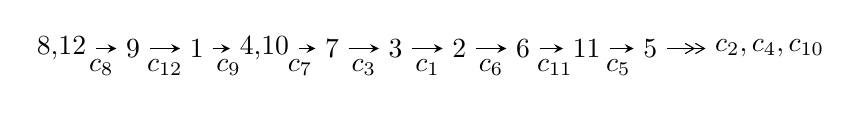
\begin{tikzpicture}[x=23pt, y=7pt]
	% node
	\node (A0) at (-1/8, 0) {8,12};
	\node (A1) at (1, 0) {9};
	\node (A2) at (2, 0) {1};
	\node (A3) at (49/16, 0) {4,10};
	\node (A4) at (33/8, 0) {7};
	\node (A5) at (41/8, 0) {3};
	\node (A6) at (49/8, 0) {2};
	\node (A7) at (57/8, 0) {6};
	\node (A8) at (65/8, 0) {11};
	\node (A9) at (73/8, 0) {5};
	\node (C1) at (1/2, -1) {$c_{8}$};
	\node (C2) at (3/2, -1) {$c_{12}$};
	\node (C3) at (5/2, -1) {$c_{9}$};
	\node (C4) at (29/8, -1) {$c_{7}$};
	\node (C5) at (37/8, -1) {$c_{3}$};
	\node (C6) at (45/8, -1) {$c_{1}$};
	\node (C7) at (53/8, -1) {$c_{6}$};
	\node (C8) at (61/8, -1) {$c_{11}$};
	\node (C9) at (69/8, -1) {$c_{5}$};
	\node (A10) at (11, 0) {$c_{2},c_{4},c_{10}$};

	% edge
	\draw[->,>=stealth]	
	(A0) edge (A1) (A1) edge (A2) (A2) edge (A3) (A3) edge (A4) (A4) edge (A5) (A5) edge (A6) (A6) edge (A7) (A7) edge (A8) (A8) edge (A9) ;
	\draw[->>,>={angle 60}]	
	(A9) edge (A10);
\end{tikzpicture} \\ 

\end{tabular} \\

\footnotetext{
The image of knot diagram is generated by the software ``\textbf{Draw programme}" developed by Andrew Bartholomew(\url{http://www.layer8.co.uk/maths/draw/index.htm\#Running-draw}), where we modified some parts for our purpose(\url{https://github.com/CATsTAILs/LinksPainter}).
}\phantom \\ \newline 
\centering \textbf{Ideals for irreducible components\footnotemark of $X_{\text{par}}$} 
 
\begin{align*}
I^u_{1}&=\langle 
9.78678\times10^{34} u^{99}+6.59298\times10^{35} u^{98}+\cdots+1.09528\times10^{33} b+7.70863\times10^{34},\\
\phantom{I^u_{1}}&\phantom{= \langle  }1.13394\times10^{35} u^{99}+7.80081\times10^{35} u^{98}+\cdots+5.47642\times10^{32} a+9.43267\times10^{34},\;u^{100}+8 u^{99}+\cdots-2 u+1\rangle \\
I^u_{2}&=\langle 
2 a^5-2 a^4+7 a^3-5 a^2+3 b+a-4,\;a^6+4 a^4+a^3+4 a^2+1,\;u-1\rangle \\
I^u_{3}&=\langle 
b,\;- u^2+a- u+1,\;u^5+u^4-2 u^3- u^2+u-1\rangle \\
\\
\end{align*}
\raggedright * 3 irreducible components of $\dim_{\mathbb{C}}=0$, with total 111 representations.\\
\footnotetext{All coefficients of polynomials are rational numbers. But the coefficients are sometimes approximated in decimal forms when there is not enough margin.}
\newpage
\renewcommand{\arraystretch}{1}
\centering \section*{I. $I^u_{1}= \langle 9.79\times10^{34} u^{99}+6.59\times10^{35} u^{98}+\cdots+1.10\times10^{33} b+7.71\times10^{34},\;1.13\times10^{35} u^{99}+7.80\times10^{35} u^{98}+\cdots+5.48\times10^{32} a+9.43\times10^{34},\;u^{100}+8 u^{99}+\cdots-2 u+1 \rangle$}
\flushleft \textbf{(i) Arc colorings}\\
\begin{tabular}{m{7pt} m{180pt} m{7pt} m{180pt} }
\flushright $a_{8}=$&$\begin{pmatrix}1\\0\end{pmatrix}$ \\
\flushright $a_{12}=$&$\begin{pmatrix}0\\u\end{pmatrix}$ \\
\flushright $a_{9}=$&$\begin{pmatrix}1\\u^2\end{pmatrix}$ \\
\flushright $a_{1}=$&$\begin{pmatrix}- u\\- u^3+u\end{pmatrix}$ \\
\flushright $a_{4}=$&$\begin{pmatrix}-207.058 u^{99}-1424.44 u^{98}+\cdots+486.994 u-172.242\\-89.3539 u^{99}-601.943 u^{98}+\cdots+192.348 u-70.3803\end{pmatrix}$ \\
\flushright $a_{10}=$&$\begin{pmatrix}- u^2+1\\- u^4+2 u^2\end{pmatrix}$ \\
\flushright $a_{7}=$&$\begin{pmatrix}70.5297 u^{99}+463.919 u^{98}+\cdots-137.456 u+47.4816\\154.340 u^{99}+987.870 u^{98}+\cdots-227.661 u+90.4459\end{pmatrix}$ \\
\flushright $a_{3}=$&$\begin{pmatrix}-173.653 u^{99}-1215.48 u^{98}+\cdots+437.871 u-154.696\\-46.3300 u^{99}-355.564 u^{98}+\cdots+185.885 u-61.7454\end{pmatrix}$ \\
\flushright $a_{2}=$&$\begin{pmatrix}194.960 u^{99}+1330.52 u^{98}+\cdots-438.893 u+154.655\\135.876 u^{99}+888.170 u^{98}+\cdots-235.645 u+90.8592\end{pmatrix}$ \\
\flushright $a_{6}=$&$\begin{pmatrix}-83.8108 u^{99}-523.951 u^{98}+\cdots+90.2049 u-42.9643\\154.340 u^{99}+987.870 u^{98}+\cdots-227.661 u+90.4459\end{pmatrix}$ \\
\flushright $a_{11}=$&$\begin{pmatrix}u^5-2 u^3+u\\u^7-3 u^5+2 u^3+u\end{pmatrix}$ \\
\flushright $a_{5}=$&$\begin{pmatrix}-9.87259 u^{99}-93.4878 u^{98}+\cdots+64.7923 u-23.7609\\155.602 u^{99}+985.103 u^{98}+\cdots-207.683 u+85.0368\end{pmatrix}$\\&\end{tabular}
\flushleft \textbf{(ii) Obstruction class $= -1$}\\~\\
\flushleft \textbf{(iii) Cusp Shapes $= -10.1896 u^{99}-65.6881 u^{98}+\cdots+19.6205 u-12.0698$}\\~\\
\newpage\renewcommand{\arraystretch}{1}
\flushleft \textbf{(iv) u-Polynomials at the component}\newline \\
\begin{tabular}{m{50pt}|m{274pt}}
Crossings & \hspace{64pt}u-Polynomials at each crossing \\
\hline $$\begin{aligned}c_{1}\end{aligned}$$&$\begin{aligned}
&u^{100}+53 u^{99}+\cdots+7 u+1
\end{aligned}$\\
\hline $$\begin{aligned}c_{2},c_{4}\end{aligned}$$&$\begin{aligned}
&u^{100}-7 u^{99}+\cdots+7 u-1
\end{aligned}$\\
\hline $$\begin{aligned}c_{3},c_{7}\end{aligned}$$&$\begin{aligned}
&u^{100}-2 u^{99}+\cdots+64 u+32
\end{aligned}$\\
\hline $$\begin{aligned}c_{5},c_{10}\end{aligned}$$&$\begin{aligned}
&u^{100}-2 u^{99}+\cdots+256 u-64
\end{aligned}$\\
\hline $$\begin{aligned}c_{6}\end{aligned}$$&$\begin{aligned}
&u^{100}-36 u^{99}+\cdots-27136 u+1024
\end{aligned}$\\
\hline $$\begin{aligned}c_{8},c_{9},c_{12}\end{aligned}$$&$\begin{aligned}
&u^{100}-8 u^{99}+\cdots+2 u+1
\end{aligned}$\\
\hline $$\begin{aligned}c_{11}\end{aligned}$$&$\begin{aligned}
&u^{100}+42 u^{99}+\cdots+49152 u+4096
\end{aligned}$\\
\hline
\end{tabular}\\~\\
\newpage\renewcommand{\arraystretch}{1}
\flushleft \textbf{(v) Riley Polynomials at the component}\newline \\
\begin{tabular}{m{50pt}|m{274pt}}
Crossings & \hspace{64pt}Riley Polynomials at each crossing \\
\hline $$\begin{aligned}c_{1}\end{aligned}$$&$\begin{aligned}
&y^{100}-5 y^{99}+\cdots-47 y+1
\end{aligned}$\\
\hline $$\begin{aligned}c_{2},c_{4}\end{aligned}$$&$\begin{aligned}
&y^{100}-53 y^{99}+\cdots-7 y+1
\end{aligned}$\\
\hline $$\begin{aligned}c_{3},c_{7}\end{aligned}$$&$\begin{aligned}
&y^{100}-36 y^{99}+\cdots-27136 y+1024
\end{aligned}$\\
\hline $$\begin{aligned}c_{5},c_{10}\end{aligned}$$&$\begin{aligned}
&y^{100}+42 y^{99}+\cdots+49152 y+4096
\end{aligned}$\\
\hline $$\begin{aligned}c_{6}\end{aligned}$$&$\begin{aligned}
&y^{100}+48 y^{99}+\cdots-43646976 y+1048576
\end{aligned}$\\
\hline $$\begin{aligned}c_{8},c_{9},c_{12}\end{aligned}$$&$\begin{aligned}
&y^{100}-88 y^{99}+\cdots+50 y+1
\end{aligned}$\\
\hline $$\begin{aligned}c_{11}\end{aligned}$$&$\begin{aligned}
&y^{100}+22 y^{99}+\cdots+461373440 y+16777216
\end{aligned}$\\
\hline
\end{tabular}\\~\\
\newpage\flushleft \textbf{(vi) Complex Volumes and Cusp Shapes}
$$\begin{array}{c|c|c}  
\text{Solutions to }I^u_{1}& \I (\text{vol} + \sqrt{-1}CS) & \text{Cusp shape}\\
 \hline 
\begin{aligned}
u &= \phantom{-}0.792365 + 0.583090 I \\
a &= -0.108287 - 1.200450 I \\
b &= \phantom{-}0.930875 - 0.648990 I\end{aligned}
 & -4.34285 - 5.74414 I & \phantom{-0.000000 } 0 \\ \hline\begin{aligned}
u &= \phantom{-}0.792365 - 0.583090 I \\
a &= -0.108287 + 1.200450 I \\
b &= \phantom{-}0.930875 + 0.648990 I\end{aligned}
 & -4.34285 + 5.74414 I & \phantom{-0.000000 } 0 \\ \hline\begin{aligned}
u &= \phantom{-}0.916971 + 0.462976 I \\
a &= -0.49303 - 1.44425 I \\
b &= \phantom{-}0.631449 - 0.855660 I\end{aligned}
 & -4.67169 + 1.91587 I & \phantom{-0.000000 } 0 \\ \hline\begin{aligned}
u &= \phantom{-}0.916971 - 0.462976 I \\
a &= -0.49303 + 1.44425 I \\
b &= \phantom{-}0.631449 + 0.855660 I\end{aligned}
 & -4.67169 - 1.91587 I & \phantom{-0.000000 } 0 \\ \hline\begin{aligned}
u &= \phantom{-}0.854924 + 0.457908 I \\
a &= -0.197120 + 0.880397 I \\
b &= \phantom{-}0.740168 + 0.665579 I\end{aligned}
 & -4.91605 - 0.63546 I & \phantom{-0.000000 } 0 \\ \hline\begin{aligned}
u &= \phantom{-}0.854924 - 0.457908 I \\
a &= -0.197120 - 0.880397 I \\
b &= \phantom{-}0.740168 - 0.665579 I\end{aligned}
 & -4.91605 + 0.63546 I & \phantom{-0.000000 } 0 \\ \hline\begin{aligned}
u &= \phantom{-}0.985240 + 0.468511 I \\
a &= -0.090625 - 0.324021 I \\
b &= -0.994121 - 0.572049 I\end{aligned}
 & -0.62795 + 2.80874 I & \phantom{-0.000000 } 0 \\ \hline\begin{aligned}
u &= \phantom{-}0.985240 - 0.468511 I \\
a &= -0.090625 + 0.324021 I \\
b &= -0.994121 + 0.572049 I\end{aligned}
 & -0.62795 - 2.80874 I & \phantom{-0.000000 } 0 \\ \hline\begin{aligned}
u &= \phantom{-}0.245788 + 0.866914 I \\
a &= -0.97785 - 1.13640 I \\
b &= \phantom{-}1.096380 - 0.741421 I\end{aligned}
 & -1.10857 - 12.68640 I & \phantom{-0.000000 } 0 \\ \hline\begin{aligned}
u &= \phantom{-}0.245788 - 0.866914 I \\
a &= -0.97785 + 1.13640 I \\
b &= \phantom{-}1.096380 + 0.741421 I\end{aligned}
 & -1.10857 + 12.68640 I & \phantom{-0.000000 } 0\\
 \hline 
 \end{array}$$\newpage$$\begin{array}{c|c|c}  
\text{Solutions to }I^u_{1}& \I (\text{vol} + \sqrt{-1}CS) & \text{Cusp shape}\\
 \hline 
\begin{aligned}
u &= \phantom{-}1.10155\phantom{ +0.000000I} \\
a &= -3.46719\phantom{ +0.000000I} \\
b &= \phantom{-}0.399241\phantom{ +0.000000I}\end{aligned}
 & -3.66615\phantom{ +0.000000I} & \phantom{-0.000000 } 0 \\ \hline\begin{aligned}
u &= \phantom{-}0.981965 + 0.530171 I \\
a &= \phantom{-}0.362459 + 0.478732 I \\
b &= \phantom{-}1.057480 + 0.710417 I\end{aligned}
 & -3.35755 + 7.75902 I & \phantom{-0.000000 } 0 \\ \hline\begin{aligned}
u &= \phantom{-}0.981965 - 0.530171 I \\
a &= \phantom{-}0.362459 - 0.478732 I \\
b &= \phantom{-}1.057480 - 0.710417 I\end{aligned}
 & -3.35755 - 7.75902 I & \phantom{-0.000000 } 0 \\ \hline\begin{aligned}
u &= \phantom{-}1.109740 + 0.184312 I \\
a &= \phantom{-}0.91419 + 1.42574 I \\
b &= \phantom{-}0.008956 + 0.667628 I\end{aligned}
 & -2.33193 - 0.86861 I & \phantom{-0.000000 } 0 \\ \hline\begin{aligned}
u &= \phantom{-}1.109740 - 0.184312 I \\
a &= \phantom{-}0.91419 - 1.42574 I \\
b &= \phantom{-}0.008956 - 0.667628 I\end{aligned}
 & -2.33193 + 0.86861 I & \phantom{-0.000000 } 0 \\ \hline\begin{aligned}
u &= \phantom{-}0.366611 + 0.787435 I \\
a &= \phantom{-}0.320115 - 0.066003 I \\
b &= \phantom{-}0.851525 + 0.600589 I\end{aligned}
 & -3.05189 + 0.94281 I & \phantom{-0.000000 } 0 \\ \hline\begin{aligned}
u &= \phantom{-}0.366611 - 0.787435 I \\
a &= \phantom{-}0.320115 + 0.066003 I \\
b &= \phantom{-}0.851525 - 0.600589 I\end{aligned}
 & -3.05189 - 0.94281 I & \phantom{-0.000000 } 0 \\ \hline\begin{aligned}
u &= \phantom{-}0.225159 + 0.838843 I \\
a &= \phantom{-}1.14281 + 1.01802 I \\
b &= -1.069060 + 0.620828 I\end{aligned}
 & \phantom{-}1.70469 - 7.47855 I & \phantom{-0.000000 } 0 \\ \hline\begin{aligned}
u &= \phantom{-}0.225159 - 0.838843 I \\
a &= \phantom{-}1.14281 - 1.01802 I \\
b &= -1.069060 - 0.620828 I\end{aligned}
 & \phantom{-}1.70469 + 7.47855 I & \phantom{-0.000000 } 0 \\ \hline\begin{aligned}
u &= \phantom{-}0.725807 + 0.461764 I \\
a &= \phantom{-}0.402301 + 0.983247 I \\
b &= -0.701413 + 0.531818 I\end{aligned}
 & -1.60708 - 1.65045 I & \phantom{-0.000000 } 0\\
 \hline 
 \end{array}$$\newpage$$\begin{array}{c|c|c}  
\text{Solutions to }I^u_{1}& \I (\text{vol} + \sqrt{-1}CS) & \text{Cusp shape}\\
 \hline 
\begin{aligned}
u &= \phantom{-}0.725807 - 0.461764 I \\
a &= \phantom{-}0.402301 - 0.983247 I \\
b &= -0.701413 - 0.531818 I\end{aligned}
 & -1.60708 + 1.65045 I & \phantom{-0.000000 } 0 \\ \hline\begin{aligned}
u &= \phantom{-}0.248644 + 0.814575 I \\
a &= \phantom{-}0.208663 + 0.177564 I \\
b &= \phantom{-}0.626377 + 0.951799 I\end{aligned}
 & -2.59413 - 6.47615 I & \phantom{-0.000000 } 0 \\ \hline\begin{aligned}
u &= \phantom{-}0.248644 - 0.814575 I \\
a &= \phantom{-}0.208663 - 0.177564 I \\
b &= \phantom{-}0.626377 - 0.951799 I\end{aligned}
 & -2.59413 + 6.47615 I & \phantom{-0.000000 } 0 \\ \hline\begin{aligned}
u &= \phantom{-}0.261461 + 0.787835 I \\
a &= -1.45679 - 1.28675 I \\
b &= \phantom{-}0.854513 - 0.596814 I\end{aligned}
 & -3.04441 - 3.78909 I & \phantom{-0.000000 } 0 \\ \hline\begin{aligned}
u &= \phantom{-}0.261461 - 0.787835 I \\
a &= -1.45679 + 1.28675 I \\
b &= \phantom{-}0.854513 + 0.596814 I\end{aligned}
 & -3.04441 + 3.78909 I & \phantom{-0.000000 } 0 \\ \hline\begin{aligned}
u &= \phantom{-}1.151430 + 0.362450 I \\
a &= \phantom{-}0.074242 + 0.848861 I \\
b &= -1.113450 - 0.084513 I\end{aligned}
 & \phantom{-}1.85816 + 1.15737 I & \phantom{-0.000000 } 0 \\ \hline\begin{aligned}
u &= \phantom{-}1.151430 - 0.362450 I \\
a &= \phantom{-}0.074242 - 0.848861 I \\
b &= -1.113450 + 0.084513 I\end{aligned}
 & \phantom{-}1.85816 - 1.15737 I & \phantom{-0.000000 } 0 \\ \hline\begin{aligned}
u &= \phantom{-}0.096928 + 0.785410 I \\
a &= \phantom{-}1.335070 + 0.123554 I \\
b &= -1.190920 + 0.174139 I\end{aligned}
 & \phantom{-}5.07427 - 5.31122 I & \phantom{-0.000000 } 0 \\ \hline\begin{aligned}
u &= \phantom{-}0.096928 - 0.785410 I \\
a &= \phantom{-}1.335070 - 0.123554 I \\
b &= -1.190920 - 0.174139 I\end{aligned}
 & \phantom{-}5.07427 + 5.31122 I & \phantom{-0.000000 } 0 \\ \hline\begin{aligned}
u &= \phantom{-}0.246130 + 0.725103 I \\
a &= -0.0848543 - 0.0498703 I \\
b &= -0.415582 - 0.737311 I\end{aligned}
 & -0.10772 - 2.32956 I & \phantom{-0.000000 } 0\\
 \hline 
 \end{array}$$\newpage$$\begin{array}{c|c|c}  
\text{Solutions to }I^u_{1}& \I (\text{vol} + \sqrt{-1}CS) & \text{Cusp shape}\\
 \hline 
\begin{aligned}
u &= \phantom{-}0.246130 - 0.725103 I \\
a &= -0.0848543 + 0.0498703 I \\
b &= -0.415582 + 0.737311 I\end{aligned}
 & -0.10772 + 2.32956 I & \phantom{-0.000000 } 0 \\ \hline\begin{aligned}
u &= \phantom{-}0.463614 + 0.601800 I \\
a &= \phantom{-}0.012853 + 0.348824 I \\
b &= -0.667970 + 0.009377 I\end{aligned}
 & -0.89045 - 2.01572 I & \phantom{-0.000000 -}0. + 5.74366 I \\ \hline\begin{aligned}
u &= \phantom{-}0.463614 - 0.601800 I \\
a &= \phantom{-}0.012853 - 0.348824 I \\
b &= -0.667970 - 0.009377 I\end{aligned}
 & -0.89045 + 2.01572 I & \phantom{-0.000000 } 0. - 5.74366 I \\ \hline\begin{aligned}
u &= -1.233550 + 0.137329 I \\
a &= -0.191271 + 0.766083 I \\
b &= -1.174580 + 0.588727 I\end{aligned}
 & -2.36040 - 4.80176 I & \phantom{-0.000000 } 0 \\ \hline\begin{aligned}
u &= -1.233550 - 0.137329 I \\
a &= -0.191271 - 0.766083 I \\
b &= -1.174580 - 0.588727 I\end{aligned}
 & -2.36040 + 4.80176 I & \phantom{-0.000000 } 0 \\ \hline\begin{aligned}
u &= \phantom{-}0.037895 + 0.743132 I \\
a &= -1.42538 + 0.35004 I \\
b &= \phantom{-}1.181760 + 0.045592 I\end{aligned}
 & \phantom{-}5.34208 - 0.12901 I & \phantom{-}4.42196 + 0. I\phantom{ +0.000000I} \\ \hline\begin{aligned}
u &= \phantom{-}0.037895 - 0.743132 I \\
a &= -1.42538 - 0.35004 I \\
b &= \phantom{-}1.181760 - 0.045592 I\end{aligned}
 & \phantom{-}5.34208 + 0.12901 I & \phantom{-}4.42196 + 0. I\phantom{ +0.000000I} \\ \hline\begin{aligned}
u &= \phantom{-}1.222230 + 0.325361 I \\
a &= -0.06233 - 1.43523 I \\
b &= \phantom{-}1.128440 - 0.155903 I\end{aligned}
 & \phantom{-}1.69954 - 3.74158 I & \phantom{-0.000000 } 0 \\ \hline\begin{aligned}
u &= \phantom{-}1.222230 - 0.325361 I \\
a &= -0.06233 + 1.43523 I \\
b &= \phantom{-}1.128440 + 0.155903 I\end{aligned}
 & \phantom{-}1.69954 + 3.74158 I & \phantom{-0.000000 } 0 \\ \hline\begin{aligned}
u &= -1.252200 + 0.185808 I \\
a &= -0.010517 - 0.443621 I \\
b &= \phantom{-}1.172560 - 0.409152 I\end{aligned}
 & -0.341204 + 0.562695 I & \phantom{-0.000000 } 0\\
 \hline 
 \end{array}$$\newpage$$\begin{array}{c|c|c}  
\text{Solutions to }I^u_{1}& \I (\text{vol} + \sqrt{-1}CS) & \text{Cusp shape}\\
 \hline 
\begin{aligned}
u &= -1.252200 - 0.185808 I \\
a &= -0.010517 + 0.443621 I \\
b &= \phantom{-}1.172560 + 0.409152 I\end{aligned}
 & -0.341204 - 0.562695 I & \phantom{-0.000000 } 0 \\ \hline\begin{aligned}
u &= \phantom{-}1.287280 + 0.148947 I \\
a &= \phantom{-}1.36344 + 0.99627 I \\
b &= \phantom{-}0.524112 + 0.620549 I\end{aligned}
 & -2.83286 - 0.52713 I & \phantom{-0.000000 } 0 \\ \hline\begin{aligned}
u &= \phantom{-}1.287280 - 0.148947 I \\
a &= \phantom{-}1.36344 - 0.99627 I \\
b &= \phantom{-}0.524112 - 0.620549 I\end{aligned}
 & -2.83286 + 0.52713 I & \phantom{-0.000000 } 0 \\ \hline\begin{aligned}
u &= \phantom{-}1.31120\phantom{ +0.000000I} \\
a &= \phantom{-}1.32824\phantom{ +0.000000I} \\
b &= \phantom{-}0.620006\phantom{ +0.000000I}\end{aligned}
 & -2.89582\phantom{ +0.000000I} & \phantom{-0.000000 } 0 \\ \hline\begin{aligned}
u &= -1.303090 + 0.182442 I \\
a &= \phantom{-}0.070720 - 1.309680 I \\
b &= -0.360096 - 0.985799 I\end{aligned}
 & -5.02002 + 0.85235 I & \phantom{-0.000000 } 0 \\ \hline\begin{aligned}
u &= -1.303090 - 0.182442 I \\
a &= \phantom{-}0.070720 + 1.309680 I \\
b &= -0.360096 + 0.985799 I\end{aligned}
 & -5.02002 - 0.85235 I & \phantom{-0.000000 } 0 \\ \hline\begin{aligned}
u &= -1.293320 + 0.293444 I \\
a &= -0.168265 + 0.657605 I \\
b &= \phantom{-}1.246390 + 0.043739 I\end{aligned}
 & \phantom{-}1.19623 + 3.85652 I & \phantom{-0.000000 } 0 \\ \hline\begin{aligned}
u &= -1.293320 - 0.293444 I \\
a &= -0.168265 - 0.657605 I \\
b &= \phantom{-}1.246390 - 0.043739 I\end{aligned}
 & \phantom{-}1.19623 - 3.85652 I & \phantom{-0.000000 } 0 \\ \hline\begin{aligned}
u &= \phantom{-}1.324190 + 0.195201 I \\
a &= \phantom{-}0.33756 + 2.77633 I \\
b &= -0.812746 + 0.636934 I\end{aligned}
 & -5.93011 - 1.80289 I & \phantom{-0.000000 } 0 \\ \hline\begin{aligned}
u &= \phantom{-}1.324190 - 0.195201 I \\
a &= \phantom{-}0.33756 - 2.77633 I \\
b &= -0.812746 - 0.636934 I\end{aligned}
 & -5.93011 + 1.80289 I & \phantom{-0.000000 } 0\\
 \hline 
 \end{array}$$\newpage$$\begin{array}{c|c|c}  
\text{Solutions to }I^u_{1}& \I (\text{vol} + \sqrt{-1}CS) & \text{Cusp shape}\\
 \hline 
\begin{aligned}
u &= -1.332070 + 0.204154 I \\
a &= \phantom{-}0.957051 + 0.408621 I \\
b &= -0.885139 + 0.235664 I\end{aligned}
 & -6.07717 + 3.20988 I & \phantom{-0.000000 } 0 \\ \hline\begin{aligned}
u &= -1.332070 - 0.204154 I \\
a &= \phantom{-}0.957051 - 0.408621 I \\
b &= -0.885139 - 0.235664 I\end{aligned}
 & -6.07717 - 3.20988 I & \phantom{-0.000000 } 0 \\ \hline\begin{aligned}
u &= \phantom{-}1.331170 + 0.220010 I \\
a &= -1.62138 - 1.30155 I \\
b &= -0.642291 - 0.912589 I\end{aligned}
 & -5.58043 - 4.45730 I & \phantom{-0.000000 } 0 \\ \hline\begin{aligned}
u &= \phantom{-}1.331170 - 0.220010 I \\
a &= -1.62138 + 1.30155 I \\
b &= -0.642291 + 0.912589 I\end{aligned}
 & -5.58043 + 4.45730 I & \phantom{-0.000000 } 0 \\ \hline\begin{aligned}
u &= -1.333540 + 0.243178 I \\
a &= -0.386912 + 1.140080 I \\
b &= \phantom{-}0.045137 + 0.949523 I\end{aligned}
 & -4.05693 + 5.10453 I & \phantom{-0.000000 } 0 \\ \hline\begin{aligned}
u &= -1.333540 - 0.243178 I \\
a &= -0.386912 - 1.140080 I \\
b &= \phantom{-}0.045137 - 0.949523 I\end{aligned}
 & -4.05693 - 5.10453 I & \phantom{-0.000000 } 0 \\ \hline\begin{aligned}
u &= \phantom{-}1.332280 + 0.250714 I \\
a &= \phantom{-}0.00784 - 2.48123 I \\
b &= \phantom{-}1.028910 - 0.614240 I\end{aligned}
 & -1.40402 - 5.45414 I & \phantom{-0.000000 } 0 \\ \hline\begin{aligned}
u &= \phantom{-}1.332280 - 0.250714 I \\
a &= \phantom{-}0.00784 + 2.48123 I \\
b &= \phantom{-}1.028910 + 0.614240 I\end{aligned}
 & -1.40402 + 5.45414 I & \phantom{-0.000000 } 0 \\ \hline\begin{aligned}
u &= -0.170952 + 0.613820 I \\
a &= \phantom{-}1.25570 - 1.69291 I \\
b &= -1.093770 - 0.670282 I\end{aligned}
 & \phantom{-}0.65018 + 7.34518 I & \phantom{-}0.51895 - 5.45269 I \\ \hline\begin{aligned}
u &= -0.170952 - 0.613820 I \\
a &= \phantom{-}1.25570 + 1.69291 I \\
b &= -1.093770 + 0.670282 I\end{aligned}
 & \phantom{-}0.65018 - 7.34518 I & \phantom{-}0.51895 + 5.45269 I\\
 \hline 
 \end{array}$$\newpage$$\begin{array}{c|c|c}  
\text{Solutions to }I^u_{1}& \I (\text{vol} + \sqrt{-1}CS) & \text{Cusp shape}\\
 \hline 
\begin{aligned}
u &= -1.323970 + 0.324415 I \\
a &= \phantom{-}0.183042 - 1.129600 I \\
b &= -1.247840 - 0.244639 I\end{aligned}
 & \phantom{-}0.61856 + 9.30284 I & \phantom{-0.000000 } 0 \\ \hline\begin{aligned}
u &= -1.323970 - 0.324415 I \\
a &= \phantom{-}0.183042 + 1.129600 I \\
b &= -1.247840 + 0.244639 I\end{aligned}
 & \phantom{-}0.61856 - 9.30284 I & \phantom{-0.000000 } 0 \\ \hline\begin{aligned}
u &= -0.099531 + 0.621357 I \\
a &= -1.48635 + 1.42762 I \\
b &= \phantom{-}1.060360 + 0.506724 I\end{aligned}
 & \phantom{-}3.11950 + 2.26469 I & \phantom{-}3.95815 - 1.35279 I \\ \hline\begin{aligned}
u &= -0.099531 - 0.621357 I \\
a &= -1.48635 - 1.42762 I \\
b &= \phantom{-}1.060360 - 0.506724 I\end{aligned}
 & \phantom{-}3.11950 - 2.26469 I & \phantom{-}3.95815 + 1.35279 I \\ \hline\begin{aligned}
u &= \phantom{-}0.113794 + 0.615400 I \\
a &= \phantom{-}0.185943 + 0.047421 I \\
b &= \phantom{-}0.088754 - 0.783282 I\end{aligned}
 & \phantom{-}0.49975 - 1.97192 I & \phantom{-}0.59201 + 5.18081 I \\ \hline\begin{aligned}
u &= \phantom{-}0.113794 - 0.615400 I \\
a &= \phantom{-}0.185943 - 0.047421 I \\
b &= \phantom{-}0.088754 + 0.783282 I\end{aligned}
 & \phantom{-}0.49975 + 1.97192 I & \phantom{-}0.59201 - 5.18081 I \\ \hline\begin{aligned}
u &= \phantom{-}1.377100 + 0.142626 I \\
a &= -1.83734 - 0.89104 I \\
b &= -0.884984 - 0.635023 I\end{aligned}
 & -5.70432 + 3.16921 I & \phantom{-0.000000 } 0 \\ \hline\begin{aligned}
u &= \phantom{-}1.377100 - 0.142626 I \\
a &= -1.83734 + 0.89104 I \\
b &= -0.884984 + 0.635023 I\end{aligned}
 & -5.70432 - 3.16921 I & \phantom{-0.000000 } 0 \\ \hline\begin{aligned}
u &= \phantom{-}1.364170 + 0.252445 I \\
a &= -0.18857 + 2.63975 I \\
b &= -1.073640 + 0.734262 I\end{aligned}
 & -4.22710 - 10.53650 I & \phantom{-0.000000 } 0 \\ \hline\begin{aligned}
u &= \phantom{-}1.364170 - 0.252445 I \\
a &= -0.18857 - 2.63975 I \\
b &= -1.073640 - 0.734262 I\end{aligned}
 & -4.22710 + 10.53650 I & \phantom{-0.000000 } 0\\
 \hline 
 \end{array}$$\newpage$$\begin{array}{c|c|c}  
\text{Solutions to }I^u_{1}& \I (\text{vol} + \sqrt{-1}CS) & \text{Cusp shape}\\
 \hline 
\begin{aligned}
u &= -1.39739 + 0.30031 I \\
a &= -0.952776 + 0.849121 I \\
b &= -0.476545 + 0.876372 I\end{aligned}
 & -5.32452 + 6.07526 I & \phantom{-0.000000 } 0 \\ \hline\begin{aligned}
u &= -1.39739 - 0.30031 I \\
a &= -0.952776 - 0.849121 I \\
b &= -0.476545 - 0.876372 I\end{aligned}
 & -5.32452 - 6.07526 I & \phantom{-0.000000 } 0 \\ \hline\begin{aligned}
u &= -1.40340 + 0.34734 I \\
a &= \phantom{-}0.28718 - 2.05993 I \\
b &= -1.100920 - 0.667509 I\end{aligned}
 & -3.46457 + 11.75370 I & \phantom{-0.000000 } 0 \\ \hline\begin{aligned}
u &= -1.40340 - 0.34734 I \\
a &= \phantom{-}0.28718 + 2.05993 I \\
b &= -1.100920 + 0.667509 I\end{aligned}
 & -3.46457 - 11.75370 I & \phantom{-0.000000 } 0 \\ \hline\begin{aligned}
u &= -1.41011 + 0.31923 I \\
a &= -0.63289 + 2.12092 I \\
b &= \phantom{-}0.931488 + 0.614497 I\end{aligned}
 & -8.35832 + 7.79358 I & \phantom{-0.000000 } 0 \\ \hline\begin{aligned}
u &= -1.41011 - 0.31923 I \\
a &= -0.63289 - 2.12092 I \\
b &= \phantom{-}0.931488 - 0.614497 I\end{aligned}
 & -8.35832 - 7.79358 I & \phantom{-0.000000 } 0 \\ \hline\begin{aligned}
u &= -1.40968 + 0.33237 I \\
a &= \phantom{-}1.20654 - 0.93297 I \\
b &= \phantom{-}0.655003 - 1.003640 I\end{aligned}
 & -7.86542 + 10.61720 I & \phantom{-0.000000 } 0 \\ \hline\begin{aligned}
u &= -1.40968 - 0.33237 I \\
a &= \phantom{-}1.20654 + 0.93297 I \\
b &= \phantom{-}0.655003 + 1.003640 I\end{aligned}
 & -7.86542 - 10.61720 I & \phantom{-0.000000 } 0 \\ \hline\begin{aligned}
u &= -0.070844 + 0.542854 I \\
a &= -0.663591 - 0.173609 I \\
b &= -0.512497 + 0.878097 I\end{aligned}
 & -1.11676 + 1.63882 I & -1.15180 - 1.38360 I \\ \hline\begin{aligned}
u &= -0.070844 - 0.542854 I \\
a &= -0.663591 + 0.173609 I \\
b &= -0.512497 - 0.878097 I\end{aligned}
 & -1.11676 - 1.63882 I & -1.15180 + 1.38360 I\\
 \hline 
 \end{array}$$\newpage$$\begin{array}{c|c|c}  
\text{Solutions to }I^u_{1}& \I (\text{vol} + \sqrt{-1}CS) & \text{Cusp shape}\\
 \hline 
\begin{aligned}
u &= -1.41825 + 0.35738 I \\
a &= -0.19419 + 2.22344 I \\
b &= \phantom{-}1.111790 + 0.773357 I\end{aligned}
 & -6.3975 + 17.0949 I & \phantom{-0.000000 } 0 \\ \hline\begin{aligned}
u &= -1.41825 - 0.35738 I \\
a &= -0.19419 - 2.22344 I \\
b &= \phantom{-}1.111790 - 0.773357 I\end{aligned}
 & -6.3975 - 17.0949 I & \phantom{-0.000000 } 0 \\ \hline\begin{aligned}
u &= -1.44935 + 0.20132 I \\
a &= -0.689559 - 0.441917 I \\
b &= -0.595033 - 0.126320 I\end{aligned}
 & -7.03499 + 4.85145 I & \phantom{-0.000000 } 0 \\ \hline\begin{aligned}
u &= -1.44935 - 0.20132 I \\
a &= -0.689559 + 0.441917 I \\
b &= -0.595033 + 0.126320 I\end{aligned}
 & -7.03499 - 4.85145 I & \phantom{-0.000000 } 0 \\ \hline\begin{aligned}
u &= -1.47182 + 0.03699 I \\
a &= -0.69034 - 1.63645 I \\
b &= -0.845947 - 0.756360 I\end{aligned}
 & -8.89073 + 2.84281 I & \phantom{-0.000000 } 0 \\ \hline\begin{aligned}
u &= -1.47182 - 0.03699 I \\
a &= -0.69034 + 1.63645 I \\
b &= -0.845947 + 0.756360 I\end{aligned}
 & -8.89073 - 2.84281 I & \phantom{-0.000000 } 0 \\ \hline\begin{aligned}
u &= -1.45081 + 0.29045 I \\
a &= \phantom{-}1.203110 - 0.440312 I \\
b &= \phantom{-}0.764537 - 0.621264 I\end{aligned}
 & -8.88672 + 2.93045 I & \phantom{-0.000000 } 0 \\ \hline\begin{aligned}
u &= -1.45081 - 0.29045 I \\
a &= \phantom{-}1.203110 + 0.440312 I \\
b &= \phantom{-}0.764537 + 0.621264 I\end{aligned}
 & -8.88672 - 2.93045 I & \phantom{-0.000000 } 0 \\ \hline\begin{aligned}
u &= -1.48199 + 0.00967 I \\
a &= \phantom{-}0.60989 - 1.90109 I \\
b &= \phantom{-}0.811592 - 0.838116 I\end{aligned}
 & -12.66580 + 1.42958 I & \phantom{-0.000000 } 0 \\ \hline\begin{aligned}
u &= -1.48199 - 0.00967 I \\
a &= \phantom{-}0.60989 + 1.90109 I \\
b &= \phantom{-}0.811592 + 0.838116 I\end{aligned}
 & -12.66580 - 1.42958 I & \phantom{-0.000000 } 0\\
 \hline 
 \end{array}$$\newpage$$\begin{array}{c|c|c}  
\text{Solutions to }I^u_{1}& \I (\text{vol} + \sqrt{-1}CS) & \text{Cusp shape}\\
 \hline 
\begin{aligned}
u &= -1.51208 + 0.04921 I \\
a &= \phantom{-}0.94033 + 1.66888 I \\
b &= \phantom{-}0.947379 + 0.764253 I\end{aligned}
 & -12.2192 + 7.4080 I & \phantom{-0.000000 } 0 \\ \hline\begin{aligned}
u &= -1.51208 - 0.04921 I \\
a &= \phantom{-}0.94033 - 1.66888 I \\
b &= \phantom{-}0.947379 - 0.764253 I\end{aligned}
 & -12.2192 - 7.4080 I & \phantom{-0.000000 } 0 \\ \hline\begin{aligned}
u &= \phantom{-}0.023033 + 0.467596 I \\
a &= \phantom{-}2.55414 - 1.74263 I \\
b &= -0.675269 - 0.423151 I\end{aligned}
 & -1.65128 - 0.65806 I & -0.515801 - 1.165772 I \\ \hline\begin{aligned}
u &= \phantom{-}0.023033 - 0.467596 I \\
a &= \phantom{-}2.55414 + 1.74263 I \\
b &= -0.675269 + 0.423151 I\end{aligned}
 & -1.65128 + 0.65806 I & -0.515801 + 1.165772 I \\ \hline\begin{aligned}
u &= -0.299051 + 0.324781 I \\
a &= -1.50249 - 0.37524 I \\
b &= -0.998992 + 0.562705 I\end{aligned}
 & -0.44144 - 4.99052 I & \phantom{-}1.47251 + 5.10258 I \\ \hline\begin{aligned}
u &= -0.299051 - 0.324781 I \\
a &= -1.50249 + 0.37524 I \\
b &= -0.998992 - 0.562705 I\end{aligned}
 & -0.44144 + 4.99052 I & \phantom{-}1.47251 - 5.10258 I \\ \hline\begin{aligned}
u &= -0.240767 + 0.153669 I \\
a &= \phantom{-}2.02139 + 0.62079 I \\
b &= \phantom{-}0.898531 - 0.269343 I\end{aligned}
 & \phantom{-}1.51367 - 0.61388 I & \phantom{-}6.21394 + 0.64261 I \\ \hline\begin{aligned}
u &= -0.240767 - 0.153669 I \\
a &= \phantom{-}2.02139 - 0.62079 I \\
b &= \phantom{-}0.898531 + 0.269343 I\end{aligned}
 & \phantom{-}1.51367 + 0.61388 I & \phantom{-}6.21394 - 0.64261 I \\ \hline\begin{aligned}
u &= \phantom{-}0.065460 + 0.176095 I \\
a &= \phantom{-}4.22561 - 2.33746 I \\
b &= -0.371284 - 0.481806 I\end{aligned}
 & -1.77841 - 0.66560 I & -4.00156 - 1.15467 I \\ \hline\begin{aligned}
u &= \phantom{-}0.065460 - 0.176095 I \\
a &= \phantom{-}4.22561 + 2.33746 I \\
b &= -0.371284 + 0.481806 I\end{aligned}
 & -1.77841 + 0.66560 I & -4.00156 + 1.15467 I\\
 \hline 
 \end{array}$$\newpage\newpage\renewcommand{\arraystretch}{1}
\centering \section*{II. $I^u_{2}= \langle 2 a^5-2 a^4+7 a^3-5 a^2+3 b+a-4,\;a^6+4 a^4+a^3+4 a^2+1,\;u-1 \rangle$}
\flushleft \textbf{(i) Arc colorings}\\
\begin{tabular}{m{7pt} m{180pt} m{7pt} m{180pt} }
\flushright $a_{8}=$&$\begin{pmatrix}1\\0\end{pmatrix}$ \\
\flushright $a_{12}=$&$\begin{pmatrix}0\\1\end{pmatrix}$ \\
\flushright $a_{9}=$&$\begin{pmatrix}1\\1\end{pmatrix}$ \\
\flushright $a_{1}=$&$\begin{pmatrix}-1\\0\end{pmatrix}$ \\
\flushright $a_{4}=$&$\begin{pmatrix}a\\-\frac{2}{3} a^5+\frac{2}{3} a^4+\cdots-\frac{1}{3} a+\frac{4}{3}\end{pmatrix}$ \\
\flushright $a_{10}=$&$\begin{pmatrix}0\\1\end{pmatrix}$ \\
\flushright $a_{7}=$&$\begin{pmatrix}\frac{2}{3} a^5+\frac{1}{3} a^4+\cdots+\frac{4}{3} a+\frac{5}{3}\\\frac{2}{3} a^5+\frac{1}{3} a^4+\cdots+\frac{4}{3} a+\frac{5}{3}\end{pmatrix}$ \\
\flushright $a_{3}=$&$\begin{pmatrix}\frac{1}{3} a^5-\frac{1}{3} a^4+\cdots-\frac{1}{3} a-\frac{2}{3}\\-\frac{1}{3} a^5+\frac{1}{3} a^4+\cdots-\frac{5}{3} a+\frac{2}{3}\end{pmatrix}$ \\
\flushright $a_{2}=$&$\begin{pmatrix}\frac{1}{3} a^5-\frac{1}{3} a^4+\cdots-\frac{1}{3} a-\frac{2}{3}\\a^5+3 a^3+2 a^2+a+1\end{pmatrix}$ \\
\flushright $a_{6}=$&$\begin{pmatrix}0\\\frac{2}{3} a^5+\frac{1}{3} a^4+\cdots+\frac{4}{3} a+\frac{5}{3}\end{pmatrix}$ \\
\flushright $a_{11}=$&$\begin{pmatrix}0\\1\end{pmatrix}$ \\
\flushright $a_{5}=$&$\begin{pmatrix}0\\\frac{2}{3} a^5+\frac{1}{3} a^4+\cdots+\frac{4}{3} a+\frac{5}{3}\end{pmatrix}$\\&\end{tabular}
\flushleft \textbf{(ii) Obstruction class $= 1$}\\~\\
\flushleft \textbf{(iii) Cusp Shapes $= -4 a^5- a^4-12 a^3-8 a^2-4 a-4$}\\~\\
\newpage\renewcommand{\arraystretch}{1}
\flushleft \textbf{(iv) u-Polynomials at the component}\newline \\
\begin{tabular}{m{50pt}|m{274pt}}
Crossings & \hspace{64pt}u-Polynomials at each crossing \\
\hline $$\begin{aligned}c_{1}\end{aligned}$$&$\begin{aligned}
&u^6-3 u^5+5 u^4-4 u^3+2 u^2- u+1
\end{aligned}$\\
\hline $$\begin{aligned}c_{2},c_{7}\end{aligned}$$&$\begin{aligned}
&u^6+u^5- u^4-2 u^3+u+1
\end{aligned}$\\
\hline $$\begin{aligned}c_{3},c_{4}\end{aligned}$$&$\begin{aligned}
&u^6- u^5- u^4+2 u^3- u+1
\end{aligned}$\\
\hline $$\begin{aligned}c_{5},c_{10},c_{11}\end{aligned}$$&$\begin{aligned}
&u^6
\end{aligned}$\\
\hline $$\begin{aligned}c_{6}\end{aligned}$$&$\begin{aligned}
&u^6+3 u^5+5 u^4+4 u^3+2 u^2+u+1
\end{aligned}$\\
\hline $$\begin{aligned}c_{8},c_{9}\end{aligned}$$&$\begin{aligned}
&(u-1)^6
\end{aligned}$\\
\hline $$\begin{aligned}c_{12}\end{aligned}$$&$\begin{aligned}
&(u+1)^6
\end{aligned}$\\
\hline
\end{tabular}\\~\\
\newpage\renewcommand{\arraystretch}{1}
\flushleft \textbf{(v) Riley Polynomials at the component}\newline \\
\begin{tabular}{m{50pt}|m{274pt}}
Crossings & \hspace{64pt}Riley Polynomials at each crossing \\
\hline $$\begin{aligned}c_{1},c_{6}\end{aligned}$$&$\begin{aligned}
&y^6+y^5+5 y^4+6 y^2+3 y+1
\end{aligned}$\\
\hline $$\begin{aligned}c_{2},c_{3},c_{4}\\c_{7}\end{aligned}$$&$\begin{aligned}
&y^6-3 y^5+5 y^4-4 y^3+2 y^2- y+1
\end{aligned}$\\
\hline $$\begin{aligned}c_{5},c_{10},c_{11}\end{aligned}$$&$\begin{aligned}
&y^6
\end{aligned}$\\
\hline $$\begin{aligned}c_{8},c_{9},c_{12}\end{aligned}$$&$\begin{aligned}
&(y-1)^6
\end{aligned}$\\
\hline
\end{tabular}\\~\\
\newpage\flushleft \textbf{(vi) Complex Volumes and Cusp Shapes}
$$\begin{array}{c|c|c}  
\text{Solutions to }I^u_{2}& \I (\text{vol} + \sqrt{-1}CS) & \text{Cusp shape}\\
 \hline 
\begin{aligned}
u &= \phantom{-}1.00000\phantom{ +0.000000I} \\
a &= -0.341164 + 0.940004 I \\
b &= -1.073950 + 0.558752 I\end{aligned}
 & -1.64493 - 5.69302 I & -3.10838 + 7.09196 I \\ \hline\begin{aligned}
u &= \phantom{-}1.00000\phantom{ +0.000000I} \\
a &= -0.341164 - 0.940004 I \\
b &= -1.073950 - 0.558752 I\end{aligned}
 & -1.64493 + 5.69302 I & -3.10838 - 7.09196 I \\ \hline\begin{aligned}
u &= \phantom{-}1.00000\phantom{ +0.000000I} \\
a &= \phantom{-}0.084211 + 0.566250 I \\
b &= \phantom{-}1.002190 + 0.295542 I\end{aligned}
 & \phantom{-}0.245672 + 0.924305 I & -1.11831 - 1.11590 I \\ \hline\begin{aligned}
u &= \phantom{-}1.00000\phantom{ +0.000000I} \\
a &= \phantom{-}0.084211 - 0.566250 I \\
b &= \phantom{-}1.002190 - 0.295542 I\end{aligned}
 & \phantom{-}0.245672 - 0.924305 I & -1.11831 + 1.11590 I \\ \hline\begin{aligned}
u &= \phantom{-}1.00000\phantom{ +0.000000I} \\
a &= \phantom{-}0.25695 + 1.72779 I \\
b &= -0.428243 + 0.664531 I\end{aligned}
 & -3.53554 + 0.92430 I & -5.77331 + 0.83820 I \\ \hline\begin{aligned}
u &= \phantom{-}1.00000\phantom{ +0.000000I} \\
a &= \phantom{-}0.25695 - 1.72779 I \\
b &= -0.428243 - 0.664531 I\end{aligned}
 & -3.53554 - 0.92430 I & -5.77331 - 0.83820 I\\
 \hline 
 \end{array}$$\newpage\newpage\renewcommand{\arraystretch}{1}
\centering \section*{III. $I^u_{3}= \langle b,\;- u^2+a- u+1,\;u^5+u^4-2 u^3- u^2+u-1 \rangle$}
\flushleft \textbf{(i) Arc colorings}\\
\begin{tabular}{m{7pt} m{180pt} m{7pt} m{180pt} }
\flushright $a_{8}=$&$\begin{pmatrix}1\\0\end{pmatrix}$ \\
\flushright $a_{12}=$&$\begin{pmatrix}0\\u\end{pmatrix}$ \\
\flushright $a_{9}=$&$\begin{pmatrix}1\\u^2\end{pmatrix}$ \\
\flushright $a_{1}=$&$\begin{pmatrix}- u\\- u^3+u\end{pmatrix}$ \\
\flushright $a_{4}=$&$\begin{pmatrix}u^2+u-1\\0\end{pmatrix}$ \\
\flushright $a_{10}=$&$\begin{pmatrix}- u^2+1\\- u^4+2 u^2\end{pmatrix}$ \\
\flushright $a_{7}=$&$\begin{pmatrix}1\\0\end{pmatrix}$ \\
\flushright $a_{3}=$&$\begin{pmatrix}u^2+u-1\\0\end{pmatrix}$ \\
\flushright $a_{2}=$&$\begin{pmatrix}u^2-1\\- u^3+u\end{pmatrix}$ \\
\flushright $a_{6}=$&$\begin{pmatrix}1\\0\end{pmatrix}$ \\
\flushright $a_{11}=$&$\begin{pmatrix}- u^4+u^2+1\\- u^4+2 u^2\end{pmatrix}$ \\
\flushright $a_{5}=$&$\begin{pmatrix}u\\u^3- u\end{pmatrix}$\\&\end{tabular}
\flushleft \textbf{(ii) Obstruction class $= 1$}\\~\\
\flushleft \textbf{(iii) Cusp Shapes $= -2 u^4-5 u^3+2 u^2+8 u-10$}\\~\\
\newpage\renewcommand{\arraystretch}{1}
\flushleft \textbf{(iv) u-Polynomials at the component}\newline \\
\begin{tabular}{m{50pt}|m{274pt}}
Crossings & \hspace{64pt}u-Polynomials at each crossing \\
\hline $$\begin{aligned}c_{1},c_{2}\end{aligned}$$&$\begin{aligned}
&(u-1)^5
\end{aligned}$\\
\hline $$\begin{aligned}c_{3},c_{6},c_{7}\end{aligned}$$&$\begin{aligned}
&u^5
\end{aligned}$\\
\hline $$\begin{aligned}c_{4}\end{aligned}$$&$\begin{aligned}
&(u+1)^5
\end{aligned}$\\
\hline $$\begin{aligned}c_{5}\end{aligned}$$&$\begin{aligned}
&u^5- u^4+2 u^3- u^2+u-1
\end{aligned}$\\
\hline $$\begin{aligned}c_{8},c_{9}\end{aligned}$$&$\begin{aligned}
&u^5+u^4-2 u^3- u^2+u-1
\end{aligned}$\\
\hline $$\begin{aligned}c_{10}\end{aligned}$$&$\begin{aligned}
&u^5+u^4+2 u^3+u^2+u+1
\end{aligned}$\\
\hline $$\begin{aligned}c_{11}\end{aligned}$$&$\begin{aligned}
&u^5+3 u^4+4 u^3+u^2- u-1
\end{aligned}$\\
\hline $$\begin{aligned}c_{12}\end{aligned}$$&$\begin{aligned}
&u^5- u^4-2 u^3+u^2+u+1
\end{aligned}$\\
\hline
\end{tabular}\\~\\
\newpage\renewcommand{\arraystretch}{1}
\flushleft \textbf{(v) Riley Polynomials at the component}\newline \\
\begin{tabular}{m{50pt}|m{274pt}}
Crossings & \hspace{64pt}Riley Polynomials at each crossing \\
\hline $$\begin{aligned}c_{1},c_{2},c_{4}\end{aligned}$$&$\begin{aligned}
&(y-1)^5
\end{aligned}$\\
\hline $$\begin{aligned}c_{3},c_{6},c_{7}\end{aligned}$$&$\begin{aligned}
&y^5
\end{aligned}$\\
\hline $$\begin{aligned}c_{5},c_{10}\end{aligned}$$&$\begin{aligned}
&y^5+3 y^4+4 y^3+y^2- y-1
\end{aligned}$\\
\hline $$\begin{aligned}c_{8},c_{9},c_{12}\end{aligned}$$&$\begin{aligned}
&y^5-5 y^4+8 y^3-3 y^2- y-1
\end{aligned}$\\
\hline $$\begin{aligned}c_{11}\end{aligned}$$&$\begin{aligned}
&y^5- y^4+8 y^3-3 y^2+3 y-1
\end{aligned}$\\
\hline
\end{tabular}\\~\\
\newpage\flushleft \textbf{(vi) Complex Volumes and Cusp Shapes}
$$\begin{array}{c|c|c}  
\text{Solutions to }I^u_{3}& \I (\text{vol} + \sqrt{-1}CS) & \text{Cusp shape}\\
 \hline 
\begin{aligned}
u &= \phantom{-}1.21774\phantom{ +0.000000I} \\
a &= \phantom{-}1.70062\phantom{ +0.000000I} \\
b &= \phantom{-0.000000 } 0\end{aligned}
 & -4.04602\phantom{ +0.000000I} & -10.7190\phantom{ +0.000000I} \\ \hline\begin{aligned}
u &= \phantom{-}0.309916 + 0.549911 I \\
a &= -0.896438 + 0.890762 I \\
b &= \phantom{-0.000000 } 0\end{aligned}
 & -1.97403 - 1.53058 I & -6.52924 + 5.40154 I \\ \hline\begin{aligned}
u &= \phantom{-}0.309916 - 0.549911 I \\
a &= -0.896438 - 0.890762 I \\
b &= \phantom{-0.000000 } 0\end{aligned}
 & -1.97403 + 1.53058 I & -6.52924 - 5.40154 I \\ \hline\begin{aligned}
u &= -1.41878 + 0.21917 I \\
a &= -0.453870 - 0.402731 I \\
b &= \phantom{-0.000000 } 0\end{aligned}
 & -7.51750 + 4.40083 I & -11.11126 - 1.16747 I \\ \hline\begin{aligned}
u &= -1.41878 - 0.21917 I \\
a &= -0.453870 + 0.402731 I \\
b &= \phantom{-0.000000 } 0\end{aligned}
 & -7.51750 - 4.40083 I & -11.11126 + 1.16747 I\\
 \hline 
 \end{array}$$\newpage
\newpage\renewcommand{\arraystretch}{1}
\centering \section*{ IV. u-Polynomials}
\begin{tabular}{m{50pt}|m{274pt}}
Crossings & \hspace{64pt}u-Polynomials at each crossing \\
\hline $$\begin{aligned}c_{1}\end{aligned}$$&$\begin{aligned}
&(u-1)^5(u^6-3 u^5+5 u^4-4 u^3+2 u^2- u+1)\\
&\cdot(u^{100}+53 u^{99}+\cdots+7 u+1)
\end{aligned}$\\
\hline $$\begin{aligned}c_{2}\end{aligned}$$&$\begin{aligned}
&((u-1)^5)(u^6+u^5+\cdots+u+1)(u^{100}-7 u^{99}+\cdots+7 u-1)
\end{aligned}$\\
\hline $$\begin{aligned}c_{3}\end{aligned}$$&$\begin{aligned}
&u^5(u^6- u^5+\cdots- u+1)(u^{100}-2 u^{99}+\cdots+64 u+32)
\end{aligned}$\\
\hline $$\begin{aligned}c_{4}\end{aligned}$$&$\begin{aligned}
&((u+1)^5)(u^6- u^5+\cdots- u+1)(u^{100}-7 u^{99}+\cdots+7 u-1)
\end{aligned}$\\
\hline $$\begin{aligned}c_{5}\end{aligned}$$&$\begin{aligned}
&u^6(u^5- u^4+\cdots+u-1)(u^{100}-2 u^{99}+\cdots+256 u-64)
\end{aligned}$\\
\hline $$\begin{aligned}c_{6}\end{aligned}$$&$\begin{aligned}
&u^5(u^6+3 u^5+5 u^4+4 u^3+2 u^2+u+1)\\
&\cdot(u^{100}-36 u^{99}+\cdots-27136 u+1024)
\end{aligned}$\\
\hline $$\begin{aligned}c_{7}\end{aligned}$$&$\begin{aligned}
&u^5(u^6+u^5+\cdots+u+1)(u^{100}-2 u^{99}+\cdots+64 u+32)
\end{aligned}$\\
\hline $$\begin{aligned}c_{8},c_{9}\end{aligned}$$&$\begin{aligned}
&((u-1)^6)(u^5+u^4+\cdots+u-1)(u^{100}-8 u^{99}+\cdots+2 u+1)
\end{aligned}$\\
\hline $$\begin{aligned}c_{10}\end{aligned}$$&$\begin{aligned}
&u^6(u^5+u^4+\cdots+u+1)(u^{100}-2 u^{99}+\cdots+256 u-64)
\end{aligned}$\\
\hline $$\begin{aligned}c_{11}\end{aligned}$$&$\begin{aligned}
&u^6(u^5+3 u^4+\cdots- u-1)(u^{100}+42 u^{99}+\cdots+49152 u+4096)
\end{aligned}$\\
\hline $$\begin{aligned}c_{12}\end{aligned}$$&$\begin{aligned}
&((u+1)^6)(u^5- u^4+\cdots+u+1)(u^{100}-8 u^{99}+\cdots+2 u+1)
\end{aligned}$\\
\hline
\end{tabular}\newpage\renewcommand{\arraystretch}{1}
\centering \section*{ V. Riley Polynomials}
\begin{tabular}{m{50pt}|m{274pt}}
Crossings & \hspace{64pt}Riley Polynomials at each crossing \\
\hline $$\begin{aligned}c_{1}\end{aligned}$$&$\begin{aligned}
&((y-1)^5)(y^6+y^5+\cdots+3 y+1)(y^{100}-5 y^{99}+\cdots-47 y+1)
\end{aligned}$\\
\hline $$\begin{aligned}c_{2},c_{4}\end{aligned}$$&$\begin{aligned}
&(y-1)^5(y^6-3 y^5+5 y^4-4 y^3+2 y^2- y+1)\\
&\cdot(y^{100}-53 y^{99}+\cdots-7 y+1)
\end{aligned}$\\
\hline $$\begin{aligned}c_{3},c_{7}\end{aligned}$$&$\begin{aligned}
&y^5(y^6-3 y^5+5 y^4-4 y^3+2 y^2- y+1)\\
&\cdot(y^{100}-36 y^{99}+\cdots-27136 y+1024)
\end{aligned}$\\
\hline $$\begin{aligned}c_{5},c_{10}\end{aligned}$$&$\begin{aligned}
&y^6(y^5+3 y^4+\cdots- y-1)(y^{100}+42 y^{99}+\cdots+49152 y+4096)
\end{aligned}$\\
\hline $$\begin{aligned}c_{6}\end{aligned}$$&$\begin{aligned}
&y^5(y^6+y^5+5 y^4+6 y^2+3 y+1)\\
&\cdot(y^{100}+48 y^{99}+\cdots-43646976 y+1048576)
\end{aligned}$\\
\hline $$\begin{aligned}c_{8},c_{9},c_{12}\end{aligned}$$&$\begin{aligned}
&((y-1)^6)(y^5-5 y^4+\cdots- y-1)(y^{100}-88 y^{99}+\cdots+50 y+1)
\end{aligned}$\\
\hline $$\begin{aligned}c_{11}\end{aligned}$$&$\begin{aligned}
&y^6(y^5- y^4+8 y^3-3 y^2+3 y-1)\\
&\cdot(y^{100}+22 y^{99}+\cdots+461373440 y+16777216)
\end{aligned}$\\
\hline
\end{tabular}
\vskip 2pc
\end{document}